% preamble
\documentclass{exam}
\usepackage[utf8]{inputenc}
\usepackage[margin=1in]{geometry}
\usepackage{amsmath}
\usepackage{amssymb}
\usepackage{siunitx}
\usepackage{graphicx}
\usepackage{multicol}
\usepackage{multirow}
\usepackage{etoolbox}
\usepackage{intcalc}
\usepackage{framed}
\usepackage{tabu}
\usepackage{tabularx}
\usepackage[dvipsnames]{xcolor}

\DeclareSIUnit \parsec {pc}
\newcommand{\match}[2]{
	\begin{tabularx}{\textwidth}{r X}
		\fillin[#1][0.5 in] & #2
	\end{tabularx}}
\newcounter{wbcount}
\newcommand{\wbelem}[1]{\stepcounter{wbcount}
	\textbf{\Alph{wbcount}} & {#1}
	\ifnumequal{0}{\intcalcMod{\value{wbcount}}{\wbcolsize}}
		{\\}
		{&}
}
\newenvironment{wordbank}[1]{
	\renewcommand*{\arraystretch}{1.5} \def\wbcolsize{#1}
	\begin{center} \begin{framed}
	\begin{tabu} to \textwidth {*{#1}{X[1,l] X[5,l]}}
	}
	{\end{tabu} \end{framed} \end{center}
}
\setlength\answerclearance{3 pt}
\newcommand{\remind}{\textcolor{red}{\rule{8pt}{8pt}}}
\newcommand{\bigO}{\mathcal{O}}

% answerkey
\newcommand{\choiceblank}[1]{
	\ifprintanswers \underline{\ \ #1\ \ }
	\else \underline{\hspace{0.40 in}}
	\fi
	\vspace{0.05 in}
}
\newcommand{\fixcolspacing}{\vspace{0pt plus 1filll}\mbox{}}
\renewcommand{\solutiontitle}{}
\unframedsolutions
\SolutionEmphasis{\color{RubineRed}}
\CorrectChoiceEmphasis{\color{RubineRed}}

%\printanswers
\pagestyle{head}
\header{MIT Invitational}{Astronomy C - Page \thepage}{Team Number:\kern .5 in}
\headrule

\begin{document}
\vspace{.25in}
\begin{center}
	\par\noindent\textbf{\large MIT Invitational, Jan 2020}
\end{center}
\begin{center}
	\par\noindent\textbf{\Huge Astronomy C}
\end{center}
\vspace{.25in}
\begin{center}
	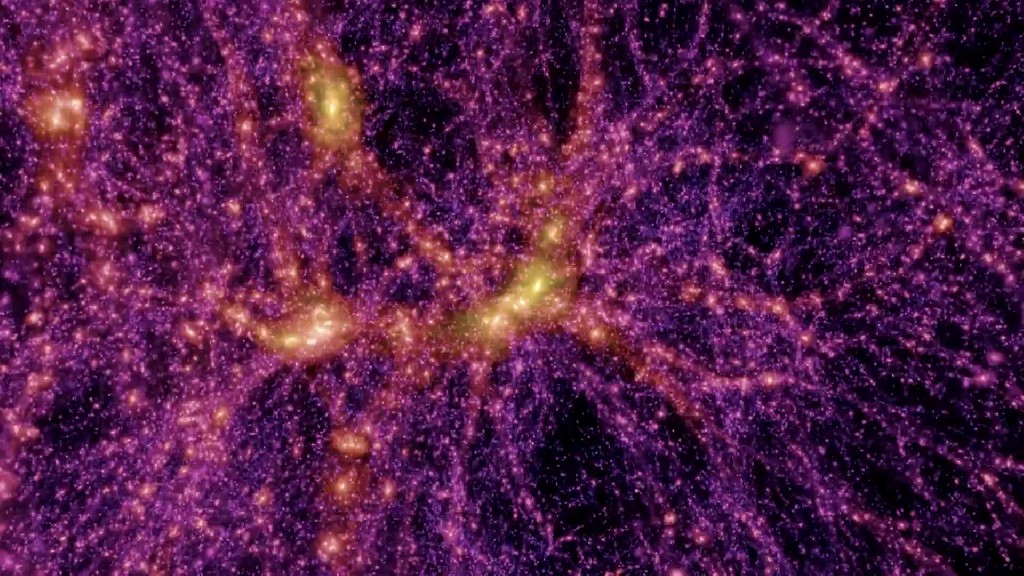
\includegraphics[width=0.7\textwidth]{images/cover.jpg}
\end{center}
\vspace{.25in}
\begin{center}
	\par
	\def\arraystretch{2}\tabcolsep=3pt
	\begin{tabular}{r r}
		\textbf{Competitors:}& \makebox[4in]{\hrulefill} \\
		\textbf{School name:}& \makebox[4in]{\hrulefill} \\
		\textbf{Team number:}& \makebox[4in]{\hrulefill} \\
	\end{tabular}
\end{center}
\vspace{.25in}
\textbf{INSTRUCTIONS}
\begin{enumerate}
    \item Please turn in \textbf{all materials} at the end of the event.
    \item You may separate the pages, but do not forget to put your \textbf{team number} at the top of every
    page.
    \item Copy your multiple choice answers to the answer page.
    \item Do not worry about significant figures. Use 3 or more in your answers, regardless
    of how many are in the question.
    \item Please \textbf{do not access the internet} during the event. If you do so, your team will be
    disqualified.
    \item Good luck! And may the stars be with you!
\end{enumerate}

\begin{center}
	\par
	\def\arraystretch{1}\tabcolsep=3pt
	\begin{tabular}{r l}
		 \textbf{{Written by:}} & Dhruva Karkada, Aditya Shah, \\
		  & Asher Noel, Antonio Frigo \\
	\end{tabular}
\end{center}
\newpage
\section*{Section A (40 pts)}
\setlength{\columnsep}{0.40 in}
\begin{multicols*}{2}
\renewcommand{\choiceshook}{\setlength{\leftmargin}{0.40 in}}
\renewcommand{\questionshook}{\setlength{\leftmargin}{0.0 in}}
\begin{questions}
\setcounter{question}{0}
\question Which image depicts NGC 2623?
	\begin{choices}
	\choice Image 4
	\choice Image 1
	\choice Image 2
	\CorrectChoice Image 7
	\end{choices}
\question Why is star formation prominent in the tails?
	\begin{choices}
	\choice Gravitational lensing causes the number of visible stars in the tails to increase
	\choice The tails are rich in WHIM, which helps cool the interstellar gas
	\CorrectChoice Gravitational interactions cause clouds of gas in the tails to be compressed
	\choice The tails contain multiple quasars, which aid in star formation
	\end{choices}
\question How does the stellar population at the nucleus of this galaxy compare to the Milky Way’s nucleus?
	\begin{choices}
	\choice It has a higher proportion of old stars than the Milky Way
	\choice There is no way to compare the stellar populations
	\choice The stellar populations have approximately the same age
	\CorrectChoice It has a higher proportion of young stars than the Milky Way
	\end{choices}
\question The apparent magnitude is observed to be $m_B=13.99$. If the galaxy is 77 million parsecs away, what is the B-band absolute magnitude?
	\begin{choices}
	\CorrectChoice -20.4 
	\choice -13.3
	\choice 2.4
	\choice 13.3
	\end{choices}
\end{questions}
\hrulefill
\begin{questions}
\setcounter{question}{4}
\question Which image depicts H1821+643?
	\begin{choices}
	\CorrectChoice Image 4
	\choice Image 8
	\choice Image 7
	\choice Image 9
	\end{choices}
\end{questions}
\vfill\null\columnbreak
\begin{questions}
\setcounter{question}{5}
\question What is the mass of the black hole in H1821+643, in solar masses?
	\begin{choices}
	\choice 5 million
	\choice 30 million
	\choice 5 billion
	\CorrectChoice 30 billion 
	\end{choices}
\question What is cooling flow?
	\begin{choices}
	\choice The flow of intergalactic gas through the cluster causes the WHIM to cool
	\choice Cold dark matter causes virgocentric flow
	\CorrectChoice Gas flows into a cluster due to the cooling of core gas
	\choice Cold gas flows out from an active galactic nucleus
	\end{choices}
\question The mass deposition rate into the center of the cluster is 5 solar masses per year. 10\% of the infalling mass is captured into the black hole’s accretion disk. Assuming that the black hole continues accreting at this steady rate, how much will the mass of the black hole increase in 1 billion years?
	\begin{choices}
	\choice 5000 solar masses
	\choice 2.5 million solar masses
	\CorrectChoice 500 million solar masses 
	\choice 2.5 billion solar masses
	\end{choices}
\end{questions}
\hrulefill
\begin{questions}
\setcounter{question}{8}
\question GW151226 was a black hole merger event. Which image depicts GW151226?
	\begin{choices}
	\CorrectChoice Image 2
	\choice Image 1
	\choice Image 7
	\choice Image 10
	\end{choices}
\question Which of these is NOT a reasonable theory for how a binary black hole system forms?
	\begin{choices}
	\choice A high-mass stellar binary system evolved into a black hole binary
	\CorrectChoice Four neutron stars undergo a double-merger to produce a black hole binary 
	\choice A black hole gravitationally captures another black hole
	\choice All of these are reasonable
	\end{choices}
\end{questions}
\vfill\null\columnbreak
\begin{questions}
\setcounter{question}{10}
\question The original black hole masses were 14.3 and 7.5 solar masses. The final black hole had mass 20.8 solar masses. How much energy was radiated away as gravitational energy? A solar mass is $\SI{2e30}{\kg}$.
	\begin{choices}
	\choice $\num{6.4e23}$ J
	\choice $\num{3.6e38}$ J
	\CorrectChoice $\num{1.8e47}$ J 
	\choice $\num{3.2e50}$ J
	\end{choices}
\question Which of the following is an accurate description of LIGO?
	\begin{choices}
	\CorrectChoice A pair of highly sensitive interferometers
	\choice An X-ray spectrograph mounted on Chandra
	\choice A vast mirror array spanning from Washington to Louisiana
	\choice A powerful electromagnetic inductor
	\end{choices}
\end{questions}
\hrulefill
\begin{questions}
\setcounter{question}{12}
\question Which image depicts M87*?
	\begin{choices}
	\CorrectChoice Image 10
	\choice Image 8
	\choice Image 6
	\choice Image 4
	\end{choices}
\question What is unique about the image?
	\begin{choices}
	\choice The light captured follows a blackbody spectrum to within 0.01\%
	\CorrectChoice It is the first picture of a black hole ever taken
	\choice It is the closest black hole to earth
	\choice The light captured was emitted only millions of years after the Big Bang
	\end{choices}
\question If the thermal radiation from the accretion disk peaks in the X-ray band, what is the approximate temperature in the disk?
	\begin{choices}
	\choice $\num{1e2}$ K
	\choice $\num{1e4}$ K
	\CorrectChoice $\num{1e7}$ K 
	\choice $\num{1e9}$ K
	\end{choices}
\end{questions}
\vfill\null\columnbreak
\begin{questions}
\setcounter{question}{15}
\question What wavelength band was this image taken in?
	\begin{choices}
	\choice Visible
	\CorrectChoice Radio
	\choice Infrared
	\choice X-ray
	\end{choices}
\end{questions}
\hrulefill
\begin{questions}
\setcounter{question}{16}
\question Which image depicts H2356-309?
	\begin{choices}
	\CorrectChoice Image 3
	\choice Image 5
	\choice Image 2
	\choice Image 1
	\end{choices}
\question What is the WHIM?
	\begin{choices}
	\choice The CMB, minus the component due to virgocentric flow
	\CorrectChoice A sparse plasma that spans the space between galaxies
	\choice The soup of primordial black holes throughout the universe
	\choice A hypothetical dark energy candidate
	\end{choices}
\question How is the WHIM different from dark matter?
	\begin{choices}
	\choice The WHIM is a specific type of dark matter
	\CorrectChoice The WHIM is baryonic, while dark matter is not
	\choice The WHIM drives the expansion of the universe, while dark matter influences matter gravitationally
	\choice Emission from the WHIM is not directly observable, while emission from dark matter is
	\end{choices}
\question What percentage of the mass-energy content of the universe is thought to be accounted for by the WHIM?
	\begin{choices}
	\choice 0.1\%
	\CorrectChoice 2.5\% 
	\choice 10\%
	\choice 25\%
	\end{choices}
\end{questions}
\vfill\null\columnbreak
\begin{questions}
\setcounter{question}{20}
\question Which image depicts the quasar 3C 273?
	\begin{choices}
	\choice Image 10
	\choice Image 4
	\choice Image 5
	\CorrectChoice Image 8
	\end{choices}
\question In which constellation is 3C 373 located?
	\begin{choices}
	\choice Draco
	\choice Bootes
	\choice Orion
	\CorrectChoice Virgo
	\end{choices}
\question If you use Hubble’s law (with $H_0=\SI{70}{\kilo\meter\per\second\per\mega\parsec}$), what is the distance to the quasar? The redshift is 0.158, and you may assume that the hubble parameter is constant ($H(t)=H_0$) during the travel time of the photons.
	\begin{choices}
	\CorrectChoice 680 Mpc 
	\choice 750 Mpc
	\choice 830 Mpc
	\choice 980 Mpc
	\end{choices}
\question A proton in the quasar jet is ejected at 99.9999\% the speed of light. Which is true about the travel time of the proton?
	\begin{choices}
	\choice It is equal to the travel distance/speed for all observers
	\CorrectChoice The proton experiences a shorter journey than the duration we measure on earth 
	\choice The proton experiences a longer journey than the duration we measure on earth
	\choice None of the above
	\end{choices}
\end{questions}
\hrulefill
\begin{questions}
\setcounter{question}{24}
\question Which image depicts MACS J0717.5+3745?
	\begin{choices}
	\choice Image 8
	\choice Image 2
	\choice Image 9
	\CorrectChoice Image 1
	\end{choices}
\end{questions}
\vfill\null\columnbreak
\begin{questions}
\setcounter{question}{25}
\question What is occurring in this DSO?
	\begin{choices}
	\CorrectChoice Four galaxy clusters have collided and merged
	\choice A neutron star merger has produced gravitational waves
	\choice Two galaxies have collided, prompting starburst
	\choice A quasar has formed from a direct-collapse black hole
	\end{choices}
\question How can we estimate the speed of the objects within the DSO?
	\begin{choices}
	\choice Use the Sunyaev-Zel'dovich effect to estimate surface density
	\CorrectChoice Examine the offset between galaxies and gas
	\choice Examine the spectal composition of the gas
	\choice Use Hubble's law to determine the peculiar motions
	\end{choices}
\question What is the Sunyaev-Zel'dovich effect?
	\begin{choices}
	\choice The distortion of spacetime due to the CMB
	\choice The distortion of spacetime due to gravitational interactions
	\choice The distortion of the CMB due to gravitational lensing
	\CorrectChoice The distortion of the CMB due to Compton scattering
	\end{choices}
\end{questions}
\hrulefill
\begin{questions}
\setcounter{question}{28}
\question Which image depicts the gamma ray burst GRB 150101B?
	\begin{choices}
	\choice Image 3
	\choice Image 6
	\choice Image 5
	\CorrectChoice Image 9
	\end{choices}
\question What is thought to have produced the gamma rays?
	\begin{choices}
	\choice The big bang
	\choice Merger of two black holes
	\choice An active galactic nucleus with an outbursting quasar
	\CorrectChoice Merger of two neutron stars
	\end{choices}
\end{questions}
\vfill\null\columnbreak
\begin{questions}
\setcounter{question}{30}
\question What important gravitational wave observation is this similar to?
	\begin{choices}
	\choice GW160420
	\CorrectChoice GW170817
	\choice GW228026
	\choice GW151226
	\end{choices}
\question The gamma rays are said to be “collimated”; what does collimated mean?
	\begin{choices}
	\CorrectChoice Travelling in the same direction (non-isotropic)
	\choice In phase with each other
	\choice Being made of baryonic particles
	\choice Having the same frequency
	\end{choices}
\end{questions}
\hrulefill
\begin{questions}
\setcounter{question}{32}
\question Which image depicts GOODS-S 29323?
	\begin{choices}
	\choice Image 3
	\CorrectChoice Image 6
	\choice Image 9
	\choice Image 10
	\end{choices}
\question When did this object form?
	\begin{choices}
	\CorrectChoice About 13 billion years ago 
	\choice About 5 billion years ago
	\choice About 13 million years ago
	\choice About 5 million years ago
	\end{choices}
\question Why is accretion not a viable mechanism for the formation of this object?
	\begin{choices}
	\choice Accretion is not consistent with CMB observations
	\choice Accretion would produce gravitational waves, which we don’t detect
	\choice We don’t see an accretion disk in X-ray observations
	\CorrectChoice The object is too massive too early to have gained mass through accretion
	\end{choices}
\end{questions}
\vfill\null\columnbreak
\begin{questions}
\setcounter{question}{35}
\question Why would JWST improve observations of direct-collapse black holes?
	\begin{choices}
	\choice JWST will be able to observe Hawking radiation from black holes
	\choice JWST will be able to observe the gravitational waves emitted by direct-collapse black holes
	\choice JWST will be able to probe the ISM for dark matter candidates
	\CorrectChoice JWST will be able to peer back in time further than current telescopes
	\end{choices}
\end{questions}
\hrulefill
\begin{questions}
\setcounter{question}{36}
\question Which image depicts MACS J1149 Lensed Star 1, also known as Icarus?
	\begin{choices}
	\choice Image 3
	\choice Image 6
	\CorrectChoice Image 5
	\choice Image 7
	\end{choices}
\question Gravitational lensing causes the apparent luminosity of the star to be magnified by a factor of 1,440,000. What is the corresponding decrease in apparent magnitude?
	\begin{choices}
	\choice 2.4
	\CorrectChoice 15.4 
	\choice 21.5
	\choice 24.0
	\end{choices}
\question If you could violate relativity and instantly teleport to the star's current location, what would you likely see? Hint: Icarus is located about 9 billion lightyears away.
	\begin{choices}
	\choice A white dwarf
	\CorrectChoice A black hole or neutron star
	\choice A blue supergiant
	\choice A type O star
	\end{choices}
\question In general relativity, the approximate deflection angle of a photon (in radians) is given in image 11. If a photon from Icarus is deflected by an angle of .01 radians, and the lensing object has mass 3 solar masses (one solar mass is \num{2e30} kg), how close did the photon pass by the lensing object?
	\begin{choices}
	\CorrectChoice 1.7 million meters 
	\choice 34 million meters
	\choice 170 million meters
	\choice 3.4 billion meters
	\end{choices}
\end{questions}
\end{multicols*}
\renewcommand{\choiceshook}{}
\renewcommand{\questionshook}{}
\raggedcolumns
\begin{multicols}{5}
\begin{enumerate}
	\setcounter{enumi}{0}
	\item \choiceblank{D}
	\item \choiceblank{C}
	\item \choiceblank{D}
	\item \choiceblank{A}
	\item \choiceblank{A}
	\item \choiceblank{D}
	\item \choiceblank{C}
	\item \choiceblank{C}
	\item \choiceblank{A}
	\item \choiceblank{B}
	\item \choiceblank{C}
	\item \choiceblank{A}
	\item \choiceblank{A}
	\item \choiceblank{B}
	\item \choiceblank{C}
	\item \choiceblank{B}
	\item \choiceblank{A}
	\item \choiceblank{B}
	\item \choiceblank{B}
	\item \choiceblank{B}
	\item \choiceblank{D}
	\item \choiceblank{D}
	\item \choiceblank{A}
	\item \choiceblank{B}
	\item \choiceblank{D}
	\item \choiceblank{A}
	\item \choiceblank{B}
	\item \choiceblank{D}
	\item \choiceblank{D}
	\item \choiceblank{D}
	\item \choiceblank{B}
	\item \choiceblank{A}
	\item \choiceblank{B}
	\item \choiceblank{A}
	\item \choiceblank{D}
	\item \choiceblank{D}
	\item \choiceblank{C}
	\item \choiceblank{B}
	\item \choiceblank{B}
	\item \choiceblank{A}
\end{enumerate}
\end{multicols}
\newpage
\section*{Section B (30 pts)}
\begin{questions}
\setcounter{question}{40}
\question \textbf{Gravitational lensing.} Use JS9 to analyze an observation of an Einstein ring around a massive lensing object.
	\begin{parts}
	\part[2] Use JS9 to determine the diameter of the ring in pixels.
		\par
		\begin{solution}[36pt]
		Accept answers between 55 - 65 pixels
		\end{solution}
	\part[2] Convert the previous answer to arcseconds. Use the ``counts in regions'' tool.
		\par
		\begin{solution}[36pt]
		Accept answers between 2.18 - 2.58 arcseconds
		\end{solution}
	\part[2] You determine that the distance to the central object is 9.2 megaparsecs. What is the diameter of the ring, in parsecs? Hint: convert the answer from part b) to radians and use the small angle approximation. (Remember: 3600 arcseconds in a degree.) Ignore cosmological effects.
		\par
		\begin{solution}[54pt]
		Accept answers between 97 - 115.1 parsecs. Partial credit: $\num{1.05e-5}$ to $\num{1.25e-5}$ radians.
		\end{solution}
	\part[2] How are the answers to parts b) and c) related to the mass of the lensing object?
		\par
		\begin{solution}[54pt]
		The mass of the lensing object affects how much light rays ``bend'' around the object. So there is a relationship between the ring radius (i.e. impact parameter), the mass, and the angular deflection.
		\end{solution}
	\part[2] What is the ratio between the apparent magnitude of the ring and the apparent magnitude of the lensing object? Use two concentric circular regions and the ``counts in regions'' tool.
		\par
		\begin{solution}[36pt]
		Accept answers between 0.4 - 0.73
		\end{solution}
	\end{parts}
\question \textbf{Galaxy observations.} Galaxy A has apparent magnitude $7.5$ and angular diameter $7^\prime$. Galaxy B has apparent magnitude $5.0$ and angular diameter $3^\circ$. Remember that there are 60 arcminutes in a degree.
	\begin{parts}
	\part[2] Find the ratio of the distances to the galaxies $d_A/d_B$ assuming their physical sizes are equal.
		\par
		\begin{solution}[54pt]
		By the small angle formula, we know that $D = \frac{\alpha d}{3438}$ where $D$ represents the physical size of the galaxy, $\alpha$ is the angular diameter in arcminutes, and $d$ is the distance to the galaxy. For ease of computation, we note that $3^\circ = 60'\cdot 3= 180'$. Hence, $\alpha_Ad_A = \alpha_Bd_B$, $\frac{d_A}{d_B} = \frac{\alpha_B}{\alpha_A} = \frac{180}{7} = 25.7.$ Thus, the ratio between their distances is 25.7:1.
		\end{solution}
	\part[2] Find the ratio of the distances to the galaxies $d_A/d_B$ assuming their absolute magnitudes are equal.
		\par
		\begin{solution}[54pt]
		Since the galaxies have the same absolute brightness, we know their absolute magnitudes $M_A = M_B$. Hence, we have the system of equations $7.5 - M = 5\log_{10}(d_A)-5$ and $5.0 - M = 5\log_{10}(d_B)-5$. Subtracting these two yields $2.5 =5\log_{10}\left(\frac{d_A}{d_B}\right).$ Solving yields $d_A/d_B = 3.16.$
		\end{solution}
	\part[2] Suppose these two galaxies are viewed along the same line of sight. What is the apparent magnitude of their combination?
		\par
		\begin{solution}[54pt]
		We will first determine the total flux observed and then convert this back into magnitudes. Note that $F_A + F_B = 10^{-0.4m_A} + 10^{-0.4m_B}.$ So $m_{AB}=-2.5\log_{10}\left(10^{-0.4m_A} + 10^{-0.4m_B}\right).$ Plugging in the given values yields $m_{AB} = 4.90.$
		\end{solution}
\newpage
	\part[2] Suppose you wanted to view galaxy A in the 1.5 GHz wavelength. Assuming a single dish, how large a diameter would you need?
		\par
		\begin{solution}[36pt]
		We know that $\theta = 1.22\frac{\lambda}{D}$ where $\theta$ is the angular resolution in radians, $\lambda$ is the wavelength, and $D$ is the diameter of the detector. We note that $7' = 0.00204$ radians and the corresponding wavelength to 1.5 GHz is $0.20$ meters. Hence $D = 120 $ meters.
		\end{solution}
	\part[2] Your answer for part d) should have been very large. What’s one technique astronomers use to circumvent this difficulty?
		\par
		\begin{solution}[36pt]
		Very-long baseline interferometry, i.e. using a bunch of radio telescopes around the earth as one large telescope.
		\end{solution}
	\end{parts}
\question \textbf{Active Galactic Nuclei.} Consider image 12, which depicts the spectral energy distribution model of an active galaxy from Della Costa \textit{et al}. (in prep.)
	\begin{parts}
	\part[2] The average dust temperature in the galaxy is about 36 K. Which of the curves likely represents the luminosity due to dust reradiation?
		\par
		\begin{solution}[18pt]
		Red curve
		\end{solution}
	\part[2] Silicates absorption troughs typically present themselves around the 10 micron region of the distribution. What Seyfert class would you expect to have a deeper trough? Explain.
		\par
		\begin{solution}[36pt]
		Type II. Seyfert II’s have more intervening dust and will result in a deeper trough
		\end{solution}
	\part[2] In order to learn more about this galaxy, you and your colleague observe it in the infrared and X-ray to try to observe its outer edges. Which would provide likely provide greater resolution images? Would it still be the best choice if there was a large amount of extinction? Explain.
		\par
		\begin{solution}[54pt]
		X-ray provides greatest resolution due to less diffraction. Not best choice since extinction affects shorter wavelengths more.
		\end{solution}
	\part[2] Often when performing estimations in astronomy, it’s useful to consider the dynamical timescale of a system to constrain an object’s physical size. It describes the minimum amount of time needed for information to travel from one end of an object to another. Consider the flux measurements shown below, taken of a galactic nucleus during an outburst of two points on the edge of the central body. What is the maximum size of the central body, in AU?
		\par
		\begin{solution}[36pt]
		To calculate the maximum size, we assume that the time difference is 24 hours, since the delay time is about 24 hours. Multiplying this by $c$ yields the total potential diameter of the central body as 173 AU.
		\end{solution}
	\part[2] To get a (very) upper bound of the central black hole's mass, we can use the upper bound calculated above as a bound for the black hole's diameter. Calculate the mass of the black hole using this bound. Is this result plausible? Explain.
		\par
		\begin{solution}[54pt]
		We find that the black hole mass $4.3\times 10^9 \text{M}_\odot.$ This is a reasonable estimate since there exist black holes with greater mass (M87’s is a great example at $7 \times 10^9 \text{M}_\odot$).
		\end{solution}
	\end{parts}
\end{questions}
\begin{table}[h]
\centering
\setlength{\tabcolsep}{5pt}
\renewcommand{\arraystretch}{1.5}
\begin{tabular}{l|l|llllll}
                            & Time (hours) & 12   & 24   & 36   & 48   & 60   & 72   \\
                            \hline
\multirow{2}{*}{Flux (mJy)} & Point A      & 12.1 & 12.0 & 12.2 & 15.6 & 16.2 & 16.4 \\
                            & Point B      & 11.9 & 16.0 & 16.3 & 17.0 & 17.1 & 17.3
\end{tabular}
\end{table}

\newpage
\section*{Section C (48 pts)}
\begin{questions}
\setcounter{question}{43}
\question \textbf{Cosmic Microwave Background.} The following questions relate to understanding the Cosmic Microwave Background (CMB).
	\begin{parts}
	\part[2] Order the following events in cosmic history: Big Bang, photon decoupling, present day, recombination, reionization. From which one of these do the current CMB photons originate?
		\par
		\begin{solution}[36pt]
		Big Bang, recombination, photon decoupling, reionization, present day \textbf{(+1)}. Photon decoupling \textbf{(+1)}.
		\end{solution}
	\part[2] Antipodal points on the CMB are $1.96d_{\textrm{hor}}$ away from each other, but they have the same temperature to within $10^{-5}$. Why is this a problem, and how is it conventionally resolved?
		\par
		\begin{solution}[54pt]
		Those regions of space should not be causally connected, so why are they in thermal equilibrium \textbf{(+1)}? Resolved with inflation \textbf{(+1)}
		\end{solution}
	\part[2] In analyzing the CMB, it's often useful to perform a multipole expansion to analyze the angular structure. What useful information is encoded in the $l=1$ multipole? Why might this explain why only multipoles with $l>1$ are plotted in image 13? (Note: in multipole expansion $0\leq l\leq\infty$.)
		\par
		\begin{solution}[54pt]
		The $l=1$ moment is the dipole moment which tells us the earth's overall motion in the universe relative to the CMB \textbf{(+1)}. This dipole anisotropy greatly skews the CMB relative to the other temperature fluctuations, so the data point would be way off the graph \textbf{(+1)}.
		\end{solution}
	\part[2] What is the relationship between a) the nonzero temperature fluctuations we see in image 13 at angular separations greater than $\approx 1^\circ$, and b) structure formation in the early universe?
		\par
		\begin{solution}[72pt]
		The fluctuations are thought to be caused by density perturbations in matter (primarily dark matter) \textbf{(+1)}. This is the Sachs-Wolfe effect. These density perturbations resulted in gravitational instabilities which gave rise to the first galaxies \textbf{(+1)}.
		\end{solution}
	\end{parts}
\question \textbf{Cosmological parameters.} The expansion of our universe (which we'll assume to be Euclidean, i.e. flat) is governed by the matter-energy content of the universe -- in particular, we care about radiation, matter, and dark energy. We quantify the present-day relative amounts of each component with density parameters $\Omega_{r,0}$, $\Omega_{m,0}$, and $\Omega_{\Lambda,0}$ respectively.
	\begin{parts}
	\part[2] Image 14 shows how a variety of observational data constrains the values of a $\Omega_{m,0}$ and $\Omega_{\Lambda,0}$. Each colored region represents the parameter values that are consistent with one type of observation. Estimate the true values of $\Omega_{m,0}$ and $\Omega_{\Lambda,0}$.
		\par
		\begin{solution}[36pt]
		$0.25 < \Omega_{m,0} < 0.35$ \textbf{(+1)} and $0.65 < \Omega_{\Lambda,0} < 0.75$ \textbf{(+1)}
		\end{solution}
	\part[2] $\Omega_{m,0}$ represents the density of all matter in the universe. Using your estimate above, what is $\Omega_{bary,0}$ (the density parameter of ``regular'' baryonic matter)?
		\par
		\begin{solution}[36pt]
		$0.035 < \Omega_{bary,0} < 0.055$ \textbf{(+2)} since about 15\% of matter is baryonic (85\% is dark matter)
		\end{solution}
\newpage
	\part[2] The super-important cosmological equation that governs the expansion of the universe is called the Friedmann equation; for a flat universe, it can be written as \[H(a) = H_0\sqrt{\frac{\Omega_{r,0}}{a^4} +\frac{\Omega_{m,0}}{a^3} + \Omega_{\Lambda,0}}\] where the Hubble parameter $H$ describes the rate of expansion of the universe as a function of the scale factor $a$. Recall that $a$ is the size of the universe relative to today, and can be used as a proxy for time (i.e. $a=0$ at the Big Bang, $a=1$ right now, and $a$ increases as time goes on). $H_0$ is our familiar Hubble constant. Using your estimate from part a), which component is most important to the dynamics of the universe today? What about in the very distant future? Justify using the flat-universe Friedmann equation.
		\par
		\begin{solution}[90pt]
		Dark energy, since its density parameter is the greatest \textbf{(+1)}. More precisely, its relative importance at scale factor $a=1$ is the greatest. In the future it's still dark energy, since its relative importance will continue to be the greatest (it's a cosmological constant, while the coefficients of all the other parameters decrease to zero as $a\to\infty$) \textbf{(+1)}.
		\end{solution}
	\part[2] The deceleration parameter $q_0$ is given by $q_0 = \Omega_{m,0}/2 - \Omega_{\Lambda,0}$. Using your estimate from part a), calculate the present deceleration of this universe, and explain its interpretation.
		\par
		\begin{solution}[54pt]
		$-0.6 < q_0 < -0.5$ \textbf{(+1)}. It tells us that the universe is accelerating in expansion \textbf{(+1)}.
		\end{solution}
	\part We can use $q_0$ to calculate distances. In particular, we can approximate the proper distance as \[d_p(z)=\frac{c}{H_0}z\left(1-z\left(\frac{1+q_0}{2}\right)\right)\] at sufficiently low $z$.
		\begin{subparts}
		\subpart[2] What is the proper distance, in lightyears, to a quasar at redshift 0.25? You can use $q_0=-0.55$.
			\par
			\begin{solution}[54pt]
			3.40 billion lightyears
			\end{solution}
		\subpart[2] What was the comoving distance to the quasar at the time the light we currently see was emitted from the quasar?
			\par
			\begin{solution}[36pt]
			The same as previous answer. Comoving distance is invariant with the expansion of the universe, and is defined as equal to the current proper distance.
			\end{solution}
		\subpart[2] The measured flux from the quasar, converted to convenient units, is \num{1.45e20} watts per square lightyear. What is the true luminosity? Account for the expansion of the universe.
			\par
			\begin{solution}[72pt]
			Convert to luminosity distance $d_L=(1+z)d_p=4.25$ billion light years \textbf{(+1)}. Use the flux relation and solve for luminosity: $L=f(4\pi d_A^2)=\num{3.3e40}$ watts \textbf{(+1)}.
			\end{solution}
		\end{subparts}
	\end{parts}
\end{questions}
\newpage
\begin{questions}
\setcounter{question}{45}
\question \textbf{Galaxy rotation.} A spiral galaxy is observed to have a rotation curve that is approximated well by the following expression: \[v(r)=250\left(1-e^{-r/R}\right)\] Where $v(r)$ is in km/s, $r$ is the radial distance from the center of the galaxy, measured in kpc, and $R$ is a constant equal to 5 kpc. Assume that the galaxy is viewed edge on.
	\begin{parts}
	\part[2] Is the rotation curve given by the expression consistent with what we could expect if the galaxy had dark matter? Why or why not?
		\par
		\begin{solution}[54pt]
		Yes, it is consistent with what we would expect. At large radii, we would expect the rotation curve to be constant if there is dark matter (+1). As $r$ increases, $e^{-r/R}$ approaches 0, so $v(r)$ approaches the constant value of 250 km/s (+1).
		\end{solution}
	\part[2] Estimate the mass of the galaxy, in solar masses, enclosed within a radius of 20 kpc.
		\par
		\begin{solution}[54pt]
		$\num{3e11}$ solar masses (+2)
		\end{solution}
	\part[2] Show that the angular frequency, $\Omega$, is constant with respect to radius near the center of the galaxy (i.e. $r \ll R$). Use the approximation $1-e^{-r/R}\approx r/R$.
		\par
		\begin{solution}[54pt]
		Using the approximation, $v(r)\approx 250 r/R$ for small values of $r$ (+1). Knowing that $\Omega r = v(r)$, $\Omega$ must be 250/$R$, which is a constant (+1).
		\end{solution}
	\end{parts}
\question \textbf{Boltzmann Distributions and Spectroscopy.} One of the most notable spectral series in Astronomy is the Balmer series, which results from electrons in the second energy level of hydrogen transitioning to higher levels upon absorbing a photon. \textit{Note: it is possible to answer part (c) without answering parts (a) or (b).}
	\begin{parts}
	\part[2] For very cool stars, a student postulates that the thermal energy in the surface of the star is not high enough to promote a significant fraction of electrons from the first energy level of hydrogen to the second. Assuming a surface temperature of 3000 Kelvin, what is the ratio of proportion of electrons in the second energy level to the first energy level (i.e. the Boltzmann Factor) throughout the surface of the star? Hint: the ionization energy of hydrogen is 13.6 eV.
		\par
		\begin{solution}[54pt]
		$\num{7e-18}$ (half credit for a guess $\pm$1 order of magnitude)
		\end{solution}
	\part[2] The student attempts to apply this logic to very hot stars, thinking that the increased thermal energy would cause all the hydrogen atoms to become ionized (i.e. be in the “infinitieth” energy level of the hydrogen atom). However, they are surprised to learn that as the temperature increases without bound to infinity, all possible energy levels of the hydrogen atom become equally populated throughout the surface of the star! Why wouldn’t the electrons preferentially occupy the highest energy states?
		\par
		\begin{solution}[72pt]
		When we are at low temperatures, states with lower energy are preferentially populated since we are constrained by the finite amount of energy available to the system. However, a system at infinite temperature would also have infinite energy, removing that constraint. So, the system has enough energy to access any state it wants. (+1) No one state is energetically preferred over another, so the electrons will distribute themselves evenly among all possible states. This configuration maximizes the entropy of the system (+1), as there are more ways to arrange electrons evenly throughout all states than putting all of them in the highest energy state.
		\end{solution}
\newpage
	\part[2] Based on the previous two parts, it is clear that the student’s idea is on the right track, but not quite correct. Briefly explain the actual reason why very hot stars and very cool stars do not display strong Balmer lines.
		\par
		\begin{solution}[72pt]
		If a star’s surface is much hotter than 10,000 K the photons coming from the star’s interior have a high enough energy to ionize many of the hydrogen atoms in the surface of the star, preventing any transitions to the second energy level (+1). In the same vein, if a star’s surface temperature if much cooler than 10,000 K, then the photons coming from the star’s interior will not have enough energy to boost many electrons from first energy level to the second energy level. Only electrons in the second energy level can absorb photons characteristic of the Balmer lines (+1). The student was generally right, but it’s the photons coming from the star’s interior that makes the difference, not the local thermal energy in the surface of the star.
		\end{solution}
	\end{parts}
\question \textbf{Galaxy collisions.} In a certain galaxy cluster, the number density of galaxies is $10^{-17}$ pc$^{-3}$. Take the average radius of each galaxy to be 25 kpc and the average speed of each member galaxy to be 1000 km/s. Unless otherwise specified, assume that the motion of the galaxies within the cluster is random and linear (i.e. gravitational interactions between the galaxies are negligible).
	\begin{parts}
	\part[2] Approximating each galaxy as a sphere, find the mean free path, in parsecs, and mean time, in years, between collisions among the galaxies in this cluster.
		\par
		\begin{solution}[54pt]
		$l = \num{5e7}$ pc (+1), $t = \num{5e10}$ years (+1)
		\end{solution}
	\part[2] In hope of getting a more accurate answer, an astronomer decides to model the galaxies not as spheres, but instead as thin disks of radius 25 kpc. One of your collaborators says that since the radius of the disk is the same as that of the sphere, the cross-sectional area is the same, resulting in no change in the mean free path or mean time between collisions. Is your collaborator correct? Why or why not?
		\par
		\begin{solution}[72pt]
		In the first model, where the galaxies are spheres, the collisions will “look” the same regardless of the orientation of the galaxies. However, then the galaxies are modelled as disks, their cross-sectional area in the direction of a collision will be different for each galaxy depending on their relative orientations (imagine the case where two disks collide edge-on as opposed to face-on as an extreme). The average cross-sectional would be smaller in the second model (+1), increasing the mean free path and mean time between collisions (+1).
		\end{solution}
	\part[2] Another astronomer decides to improve on the original model by including an attractive gravitational force between the galaxies, still modelling them as spheres of radius 25 kpc. How would this affect the mean free path and mean time between galaxy collisions? Is the effect of the gravitational attraction more significant at higher or lower average velocities? Explain your answers qualitatively.
		\par
		\begin{solution}[54pt]
		An attractive force between the galaxies would reduce the mean free path and mean time between collisions (+1). This effect will be more pronounced at lower velocities, when the attractive force between the particles results in a larger fractional change in the velocity ($\Delta v/\langle v\rangle$) of each individual galaxy (+1).
		\end{solution}
	\end{parts}
\end{questions}
\newpage
\begin{questions}
\setcounter{question}{48}
\question[8] \textbf{Research techniques.} Computational methods and simulations are integral to most realms of modern astrophysics research. For the following eight scenarios, pick a simulation or research technique from the list below that would be best suited to support or reject a related hypothesis.
	\begin{parts}
	\part To simulate and analyze the dynamics of a galaxy merger.
		\par
		\begin{solution}[18pt]
		N-body
		\end{solution}
	\part To survey and classify recent Gaia data to catalog elliptical galaxies.
		\par
		\begin{solution}[18pt]
		Neural Network
		\end{solution}
	\part To research cold dark matter’s role in galaxy formation.
		\par
		\begin{solution}[18pt]
		SPH
		\end{solution}
	\part To predict the neutrino extinction of the intergalactic medium.
		\par
		\begin{solution}[18pt]
		Monte Carlo
		\end{solution}
	\part To identify filaments of the cosmic web in sky surveys.
		\par
		\begin{solution}[18pt]
		Neural Network
		\end{solution}
	\part To model the gravitational dynamics of a globular cluster.
		\par
		\begin{solution}[18pt]
		N-body
		\end{solution}
	\part To explore the role of feedback in producing large scale structures.
		\par
		\begin{solution}[18pt]
		SPH
		\end{solution}
	\part To model the creation of jets in long gamma ray bursts.
		\par
		\begin{solution}[18pt]
		GRMHD
		\end{solution}
	\end{parts}
\end{questions}
Some research techniques.
\begin{itemize}
    \item \textbf{General Relativistic magnetohydrodynamics (GRMHD):} simulations that solve five equations of general relativity while studying the magnetic properties and behavior of electrically conducting fluids. 
    \item \textbf{N-body:} a simulation of a dynamical system of particles, usually influenced by physical forces.
    \item \textbf{Monte-Carlo:}  a simulation that uses randomness to model the probability of different outcomes.
    \item \textbf{Neural Network:} a model that learns from training data. 
    \item \textbf{Smoothed-Particle Hydrodynamics (SPH):} a computational method used for simulating the mechanics of fluid flows.
\end{itemize}
\end{document}
